%-------------------------------------------------------------------------------
\tikzset{fl/.style={ draw, fill = gray,rectangle,minimum size=3mm}}
\tikzset{sub/.style={ draw, shape border rotate=90, isosceles triangle,minimum size=8mm,yshift=-8mm}}
%-------------------------------------------------------------------------------
%-------------------------------------------------------------------------------
\chapter{Codage de Huffman}
%-------------------------------------------------------------------------------
%-------------------------------------------------------------------------------
\thispagestyle{empty}
%-------------------------------------------------------------------------------
%-------------------------------------------------------------------------------
\begin{abstract}
Pour coder les chaînes de caractères, le code le plus répandu est le code ASCII\footnote{\sc American Standard
Computer Information Interchange}. Dans ce code, chaque caractère est codé par un octet, c'est-à-dire par un mot de 8 bits. Un texte de $n$ caractères est donc codé sur $8n$ bits.

Il est parfois utile de comprimer le codage : une méthode possible consiste à coder les caractères les plus fréquents des mots de longueur inférieure à 8, alors que d'autres seront codés par des mots plus longs. L'idée est que la longueur
moyenne d'un texte de $n$ caractères pourrait être alors strictement inférieure à $8n$.

Une telle méthode est proposée par le codage de Huffman.
\end{abstract}
%-------------------------------------------------------------------------------
%-------------------------------------------------------------------------------
%-------------------------------------------------------------------------------
\section{Arbre de Huffman}
%-------------------------------------------------------------------------------
%-------------------------------------------------------------------------------
%-------------------------------------------------------------------------------
Pour qu'un codage soit utilisable il faut que le texte codé soit décodable.

La méthode de Huffman consiste à définir un code qui soit préfixe, c'est à dire qu'aucun code d'une lettre n'est le préfixe du code d'une autre lettre.

Par exemple, le code $a\mapsto 01$, $b\mapsto 101$, $c\mapsto 00$, $d\mapsto 1001$, $e\mapsto 11$, $f\mapsto 1000$ est préfixe et on peut décoder $0110001001101110100$\footnote{"afdbeac"}

\medskip

On passe d'un caractère à son code ASCII par le biais de la fonction \type{Char.code} ou \type{int\_of\_char}, dont l'inverse est  \type{Char.chr} ou \type{char\_of\_int}. 

{\bf N.B.} Les versions récentes de OCaml utilisent le codage UTF les fonctions ci-dessus ne sont utilisables que pour les codes ASCII de 0 à 127. 

Il faudra donc exclure les lettres accentuées et autres caractères spécifiques. 

Les tableaux indexés par les codes pourront se limiter à une longueur 128.

\medskip  

Un tel code est représentable par un arbre $T$ dont les feuilles sont étiquetées par les lettres et le code d'une lettre $a$, $C(a)$, est donné par le chemin qui relie la racine de $T$ à la feuille d'étiquette $a$, une descente à gauche ou à droite correspondant respectivement à un caractère 0 ou 1. Le code défini ci-dessus est associé à l'arbre dessiné ci-après.

On supposera également que les nœuds internes des arbres ont exactement deux fils.

%-------------------------------------------------------------------------------
\begin{center}
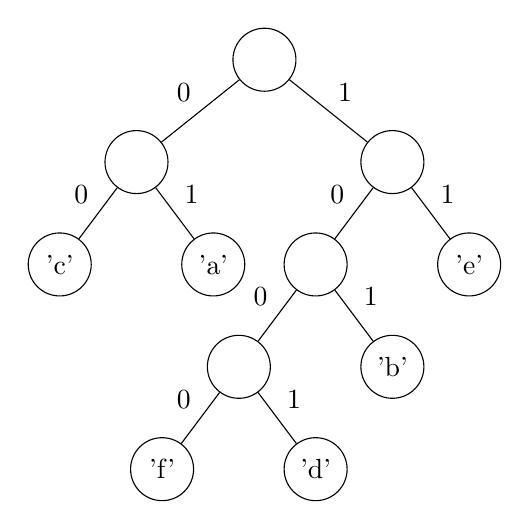
\begin{tikzpicture}[scale  = 0.65]
\tikzstyle{n}=[draw, circle, minimum size=8mm]
\node[n](cafdbe)   at ( 0,  0) {} ;
\node[n](ca)       at (-2.5, -2) {} ;
\node[n](fdbe)     at ( 2.5, -2) {} ;
\node[n](c)        at (-4, -4) {'c'} ;
\node[n](a)        at (-1, -4) {'a'} ;
\node[n](fdb)      at ( 1, -4) {} ;
\node[n](e)        at ( 4, -4) {'e'} ;
\node[n](fd)       at (-0.5, -6) {} ;
\node[n](b)        at ( 2.5, -6) {'b'} ;
\node[n](f)        at (-2, -8) {'f'} ;
\node[n](d)        at ( 1, -8) {'d'} ;

\draw (cafdbe) -- node[above left]  {0} (ca) ;
\draw (cafdbe) -- node[above right] {1} (fdbe) ;
\draw (ca)     -- node[above left]  {0} (c) ;
\draw (ca)     -- node[above right] {1} (a) ;
\draw (fdbe)   -- node[above left]  {0} (fdb) ;
\draw (fdbe)   -- node[above right] {1} (e) ;
\draw (fdb)    -- node[above left]  {0} (fd) ;
\draw (fdb)    -- node[above right] {1} (b) ;
\draw (fd)     -- node[above left]  {0} (f) ;
\draw (fd)     -- node[above right] {1} (d) ;
\end{tikzpicture} 
\end{center}
%--------------------------------------------------------------------------
On ajoute aussi un poids (entier) à chaque nœud. On définit donc le type de données
\begin{lstlisting}
type arbre = F of int * char | N of arbre * int * arbre;;
\end{lstlisting}
Le poids d'un arbre sera le poids de sa racine.
%--------------------------------------------------------------------------
%--------------------------------------------------------------------------
\begin{Exercise}[title = Poids]\it 
Écrire une fonction \type{poids : arbre -> int} qui renvoie le poids d'un arbre.
\end{Exercise}
%--------------------------------------------------------------------------
\begin{Answer}
\begin{lstlisting}
let poids a = 
  match a with 
  |F(k, c) -> k
  |N(g, k, d) -> k;;
\end{lstlisting}
\end{Answer}
%--------------------------------------------------------------------------%--------------------------------------------------------------------------
Le codage est adapté au texte à compacter.

L'arbre associé à ce codage est obtenu de la façon suivante.
%--------------------------------------------------------------------------
\begin{enumerate}
  \item En lisant une première fois le texte, on accorde à chaque caractère un poids : le nombre d'apparitions du caractère dans le texte. Ces poids sont stockés dans un tableau de longueur $128$.
%--------------------------------------------------------------------------
  \item On construit une file de priorité initiale, dont les éléments sont les
arbres de Huffman, réduits à des feuilles \type{N(char, poids)}, pour chaque lettre : l'{\bf alphabet pondéré}.
%--------------------------------------------------------------------------
\item Tant que la file contient au moins deux arbres :
%--------------------------------------------------------------------------
\begin{enumerate}
  \item on retire les deux arbres de plus faibles poids, $h_1$ et $h_2$ de poids respectifs $w_1$ et $w_2$,
  \item on construit un nouvel arbre $h$ (de Huffman) dont les sous-arbres gauche et droit sont $h_1$ et $h_2$ et de poids $w_1+w_2$,
  \item on ajoute ce nouvel arbre dans la file de priorité.
\end{enumerate}
%--------------------------------------------------------------------------
\item Quand la file est réduite à un unique arbre, on renvoie cet arbre. Le code associé est le {\bf code de Huffman} du texte (on admet que ce code est bien optimal).
\end{enumerate}
%--------------------------------------------------------------------------

Le nombre d'éléments dans la file d'attente n'est pas très élevé, on se contentera de coder celle-ci par une liste triée par poids croissant.
%--------------------------------------------------------------------------
%--------------------------------------------------------------------------
\begin{Exercise}[title = Insertion]\it 
Écrire une fonction \type{inserer : arbre -> arbre list -> arbre list} qui ajoute un arbre à une liste d'arbres ; on supposera que la liste initiale est triée par ordre croissant de poids et la liste renvoyée le sera également.
\end{Exercise}
%--------------------------------------------------------------------------
\begin{Answer}
\begin{lstlisting}
let rec inserer a liste = 
  match liste with
  |[] -> [a]
  |t::reste when poids(a) > poids(t) -> t :: (inserer a reste)
  |_ -> a::liste;;
\end{lstlisting}
\end{Answer}
%--------------------------------------------------------------------------
%--------------------------------------------------------------------------
\begin{Exercise}[title = Calcul des poids, label =ques:tableOcc]\it 
Écrire une fonction \type{occ : string -> int array} qui calcule le tableau des occurrences des 128 caractères dans un texte.
\end{Exercise}
%--------------------------------------------------------------------------
\begin{Answer}
\begin{lstlisting}
let occ texte = 
  let t = Array.make 128 0 in
  for i = 0 to (String.length u -1) do
      let k = Char.code u.[i] in
      t.(k) <- t.(k) + 1 done;
 t;;
\end{lstlisting}
\end{Answer}
%--------------------------------------------------------------------------%--------------------------------------------------------------------------
\begin{Exercise}[title = Calcul de l'alphabet]\it 
Écrire une fonction \type{alphabet : int array -> arbre list} qui calcule l'alphabet pondéré associé à tableau des poids.

On ne mettra dans la liste que les caractères qui ont une fréquence non nulle.
\end{Exercise}
%--------------------------------------------------------------------------
\begin{Answer}
\begin{lstlisting}
let alphabet t = 
 let alphabet = ref [] in
 for k = 0 to 255 do
   if t.(k)<>0 
   then alphabet := inserer (F(t.(k), Char.chr k)) 
                            !alphabet done;      
 !alphabet;;
\end{lstlisting}
\end{Answer}
%--------------------------------------------------------------------------
%--------------------------------------------------------------------------
\begin{Exercise}[title = Calcul de l'arbre]\it 
Écrire une fonction \type{arbre\_huffman : arbre list -> arbre} qui, appliquée à un alphabet pondéré, renvoie l'arbre du code de Huffman qui lui est associé.
\end{Exercise}
%--------------------------------------------------------------------------
\begin{Answer}
\begin{lstlisting}
let rec arbre_huffman alphabet = 
  match alphabet with
  |[] -> failwith "Le texte est-il vide ?"
  |[a] -> a
  |a::b::q -> let t = N(a, (poids a) + (poids b), b) in
              arbre_huffman (inserer t q);;
\end{lstlisting}
\end{Answer}
%--------------------------------------------------------------------------
%--------------------------------------------------------------------------
\newpage 

L'arbre associé à un texte sera donc calculé par 
\begin{lstlisting}
let t = arbre_huffman (alphabet (poids texte));;
\end{lstlisting}

%--------------------------------------------------------------------------
%--------------------------------------------------------------------------
\begin{Exercise}[title = Table de codage]\it 
Écrire une fonction \type{table\_codes} qui, appliquée à un arbre, renvoie le tableau de longueur
128 dont la $i$-ème entrée contient le code $C(a)$ où $a$ est le caractère de code ASCII $i$.
Le code sera codé sous la forme d'une chaîne de caractères \type{'0'} ou \type{'1'} et sera égal à la chaîne vide si $a$ n'est pas codé par $C$.
\end{Exercise}
%--------------------------------------------------------------------------
\begin{Answer}
On définit une fonction auxiliaire qui ajoute une chaîne (qui sera \type{"0"} ou \type{"1"}) à toutes les chaînes d'une liste (les codes d'un fils).
\begin{lstlisting}
let rec prefixe pref liste =
  match liste with
  |[] -> []
  |(car, ch)::reste -> (car, pref^ch)::(prefixe pref reste);;
\end{lstlisting}

On peut aussi écrire
\begin{lstlisting}
let prefixe pref = List.map (fun (car, ch) -> (car, pref^ch));;
\end{lstlisting}

On commence par lire l'arbre pour obtenir la liste des couples caractère-code.
\begin{lstlisting}
let rec lecture arbre = 
  match arbre with
  |F(_, ch) -> [(ch, ""]
  |N(g, _, d) -> (prefixe "0" (lecture g))
                @(prefixe "1" (lecture d));;
\end{lstlisting}
On peut alors remplir un tableau

\begin{lstlisting}
let table_code arbre =
  let liste = lecture arbre in
  let c = Array.make 128 "" in
  let rec appliquer liste = 
    match liste with
    |[] -> ()
    |(car, code)::reste -> let k = Char.code car in
                           c.(k) <- code;
                           appliquer reste in
  appliquer liste;
  c;;
\end{lstlisting}

On peut aussi écrire
\begin{lstlisting}
let table_code arbre =
  let liste = lecture arbre in
  let c = Array.make 128 "" in
  List.iter (fun (a, b) -> c.(Char.code a) <- b) liste;
  c;;
\end{lstlisting}

\end{Answer}
%-------------------------------------------------------------------------------
%-------------------------------------------------------------------------------
%-------------------------------------------------------------------------------
\section{Codage-décodage}
%-------------------------------------------------------------------------------
%-------------------------------------------------------------------------------
%-------------------------------------------------------------------------------
\begin{Exercise}[title = Codage avec table]\it 
Écrire une fonction \type{coder\_table}, qui prend en argument une table de
code et une liste de caractères et qui renvoie le texte codé. 
\end{Exercise}
%--------------------------------------------------------------------------
\begin{Answer}
\begin{lstlisting}
let coder_table table  texte =
  let n = Array.length texte in
  let comp = ref "" in
  for i = 0 to (n-1) do 
    let k = Char.code texte.[i] in
    comp := !comp^table.(k) done;
  !comp;;
\end{lstlisting}
\end{Answer}
%--------------------------------------------------------------------------
%--------------------------------------------------------------------------
\begin{Exercise}[title = Codage du texte]\it 
En déduire une fonction qui, à partir d'un texte, renvoie le couple formé de la table des occurrences (voir question \ref{ques:tableOcc}) et du texte compacté.
\end{Exercise}
%--------------------------------------------------------------------------
\begin{Answer}
\begin{lstlisting}
let codage texte =
  let t = occ texte in
  let arbre  = arbre_huffman (alphabet t) in
  let table = table_code (lecture arbre) in
  t, (codage_table table texte);;
\end{lstlisting}
\end{Answer}
%--------------------------------------------------------------------------
%--------------------------------------------------------------------------
\begin{Exercise}[title = Analyse]\it 
Quel défaut présente l'algorithme de Huffman ?

Proposer une fonction qui détermine l'efficacité de la compression. 

On notera que, pour mesurer l'efficacité, la longueur de la chaîne de 0 et 1 peut être divisé par 8 car on pourra coder les 0/1 sur un seul bit au lieu d'un octet. 
\end{Exercise}
%--------------------------------------------------------------------------
\begin{Answer}
On doit lire le texte deux fois, cela implique que l'on doit connaître tout le texte {\bf avant} de le compresser. On ne peut donc pas compresser "à la volée".
\begin{lstlisting}
let taux_compression texte = 
  let _, comp = codage text in
  100*(String.length v)/(String.length u)/8;;
\end{lstlisting}
Donne le pourcentage de compression (un entier).
\end{Answer}
%--------------------------------------------------------------------------
%--------------------------------------------------------------------------
\begin{Exercise}[title = Décodage d'une lettre]\it 
Écrire une fonction prenant en argument un arbre de Huffman, une chaîne de 0 et 1 et un indice valide de cette chaîne et qui retourne le caractère décodé dont le codage commence à l'indice ainsi que l'indice du premier indice non utilisé.
\end{Exercise}
%--------------------------------------------------------------------------
\begin{Answer}
\begin{lstlisting}
let decode huff ch i =
  let rec descente arbre ind =
     match arbre with
     |F(_, car) -> car
     |N(g, _, _) when ch.[ind] = '0' -> descente g (ind + 1)
     |N(_, _, d) -> descente d (ind + 1) in
  descente huff i;;
\end{lstlisting}
\end{Answer}
%--------------------------------------------------------------------------
%--------------------------------------------------------------------------
\begin{Exercise}[title = Décodage]\it 
En déduire une fonction \type{decode : int array -> string -> string} qui retourne le texte décodé à partir de la table des occurrences et du texte codé.

\end{Exercise}
%--------------------------------------------------------------------------
\begin{Answer}
\begin{lstlisting}
let decode t comp = 
  let texte = ref "" in
  let n = String.length comp in
  let ind = ref 0 in
  let a = arbre_huffman (alphabet t) in
  while !ind < n do
    let car, k = decode a comp !ind in
    ind := k;
    texte := !texte ^ (Char.escaped car) done;
  !texte;;
\end{lstlisting}
\end{Answer}
%--------------------------------------------------------------------------%--------------------------------------------------------------------------
\type{Char.escaped car} convertit un caractère en une chaîne de longueur 1.
%--------------------------------------------------------------------------
%--------------------------------------------------------------------------
\begin{Exercise}[title = Codage compacté]\it 
Coder un texte sous forme compactée en une chaîne de caractères.

Pour simplifier on n'utilisera que les caractères de code ASCII entre 0 et 127 donc on regroupera les chiffres 7 par 7, ce qui donne un taux de compression moins avantageux.

Pour gérer une taille qui n'est pas un multiple de 7 on pourra ajouter un caractère sentinelle au texte original, par exemple \type{Char.chr 0} et ajouter des caractères 0 à la chaîne de 0 et 1 pour obtenir une longueur multiple de 7.
\end{Exercise}
%--------------------------------------------------------------------------
\begin{Answer}
\begin{lstlisting}
\end{lstlisting}
\end{Answer}
%--------------------------------------------------------------------------%--------------------------------------------------------------------------
%-------------------------------------------------------------------------------
% \section{Fichiers textes}
% %-------------------------------------------------------------------------------
% %-------------------------------------------------------------------------------
% %-------------------------------------------------------------------------------
%
% %--------------------------------------------------------------------------
% %--------------------------------------------------------------------------
% \begin{Exercise}[title = ]\it 
%
% \end{Exercise}
% %--------------------------------------------------------------------------
% \begin{Answer}
% \begin{lstlisting}
%
% \end{lstlisting}
% \end{Answer}
% %--------------------------------------------------------------------------%--------------------------------------------------------------------------
%

%-------------------------------------------------------------------------------
%-------------------------------------------------------------------------------
%-------------------------------------------------------------------------------
